After completing the Bayesian estimation for parameter $A$, a natural question arises: 
Does the extended survival model, under the parametrization $(\lambda, A)$, remain theoretically identifiable and consistent with the original exponential survival model?
To address this, we first establish the identifiability of $(\lambda, A)$ within this model, and then examine how the joint posterior structure and marginalization of $A$ reflect consistency with the baseline model. 

\subsubsection{Identifiability}
Once the new parameter $A$ is introduced, the first question is whether the model indexed by $(\lambda, A)$ remains identifiable. That is, whether distinct parameter values induce distinct distributions of the observables.
\begin{definition}\textbf{(Identifiability)}. Consider a statistical model $\mathcal P=\{P_\theta:\theta\in\Theta\}$, where $\theta$ is the parameter indexing the family and $\Theta$ may be finite- or infinite-dimensional. We say that $\mathcal P$ is identifiable under the parametrization $\theta$ if the following condition holds~\cite{lehmann1998theory, van2000asymptotic}
\begin{equation}
    P_{\theta_1}=P_{\theta_2}\ \Longrightarrow\ \theta_1=\theta_2,\qquad \forall\,\theta_1,\theta_2\in\Theta .
\end{equation}
Equivalently, the mapping $\theta\mapsto P_\theta$ is injective~\cite{lehmann1998theory}.
\end{definition}
%%%%%%%%%%%%%%%%%%%%%%%%%%%%%%%%
\begin{proof}
The observed data are pairs $(Y,\delta)$ with $Y=\min(T,C)$ and $\delta=\mathbf 1\{T\le C\}$. 
Under $T\sim\text{Exp}(\lambda)$, independent censoring with horizon $A$, and uniform entry, 
the distribution $P_\psi$ with $\psi=(\lambda,A)$ is characterized by two component densities
\begin{equation}
f_0(y\mid\lambda,A)=\frac{1}{A}\,e^{-\lambda y}, \quad 0\le y\le A, \qquad (\delta=0),
\end{equation}
\begin{equation}
f_1(y\mid\lambda,A)=\lambda e^{-\lambda y}\Big(1-\tfrac{y}{A}\Big), \quad 0<y<A, \qquad (\delta=1).
\end{equation}
\textbf{Identifiability of $A$}. 
For censored observations $(\delta=0)$, the density $f_0$ has support $[0,A]$, depending only on $A$. Suppose $P_{\lambda_1,A_1}=P_{\lambda_2,A_2}$. If $A_1\ne A_2$, without loss of generality let $A_1<A_2$, 
and consider $B=(A_1,(A_1+A_2)/2]$. Then
\begin{equation}
P_{\lambda_1,A_1}(Y\in B,\delta=0)=\int_B \tfrac{1}{A_1}e^{-\lambda_1 y}\,dy=0,
\end{equation}
while
\begin{equation}
P_{\lambda_2,A_2}(Y\in B,\delta=0)=\int_B \tfrac{1}{A_2}e^{-\lambda_2 y}\,dy>0.
\end{equation}
This contradiction implies $A_1=A_2$. Hence, the parameter $A$ is identifiable.

\textbf{Identifiability of $\lambda$.}
Fixing $A$, the support is identical across all parameter values, so differences must arise from the shape of the distribution. Since $P_\psi$ is fully determined by the pair $(f_0,f_1)$, any functional transformation thereof also characterizes the model. In particular, the ratio of event to censoring densities,
\begin{equation}
R(y;\lambda,A)=\frac{f_1(y\mid\lambda,A)}{f_0(y\mid\lambda,A)}=\lambda(A-y), \qquad 0<y<A ,
\end{equation}
provides a convenient summary to examine the role of $\lambda$. This ratio is a deterministic linear function in $y$, with slope $-\lambda$ and intercept $\lambda A$. Since $A$ has already been identified in step 1, equality of ratios implies $\lambda_1=\lambda_2$. 

Therefore, both parameters are uniquely determined by the distribution of $(Y,\delta)$, and the model is identifiable in $(\lambda,A)$.
\end{proof}

\subsubsection{Grid-based Contour Analysis of the Joint Posterior}

To further examine how identifiability appears in finite-sample settings, we characterize the shape of the joint posterior distribution and visualize its structure numerically.

As shown in Equation~\eqref{A_post} of Section~\ref{A_bayes}, we adopt the same prior for $\lambda$ as in Section~\ref{指数模型贝叶斯推断过程} (the exponential model case), to ensure comparability and to facilitate the later marginalization check in Section~\ref{边际化章节}. For $A$, we use a uniform prior $\mathrm{Unif}(y_{\max}, y_{\max}+500)$, which is relatively broad but still consistent with the constraints discussed in Section~\ref{Impact of A}: the survey duration cannot extend indefinitely (e.g., 1000 months).

Under this setting, the log-posterior is
\begin{align}
\log p(\lambda, A \mid \mathcal D)
&= \text{const}
   + \Big(\sum_{i=1}^n \delta_i\Big)\log \lambda
   - \lambda \sum_{i=1}^n y_i \nonumber\\[6pt]
&\quad + \sum_{i:\,\delta_i=1}\log(A-y_i)
   - n \log A
   + \log \pi_\lambda(\lambda) \nonumber \\[6pt]
&\quad + \log \pi_A(A) + \log \mathbf 1\{A \ge \max_i y_i\}.
\end{align}
Since the model involves only two parameters $(\lambda, A)$, we approximate the posterior on a two-dimensional grid~\cite{mcelreath2021grid}. At each grid point $(\lambda_i, A_j)$, we evaluate the log-posterior, exponentiate, and normalize to obtain weights~\cite{ORMEROD201145,mcelreath2021grid}
\begin{equation}
    w_{ij} \;\propto\; \exp\!\Bigl(\log p(\lambda_i, A_j \mid \mathcal D)\Bigr), \qquad \tilde w_{ij} \;=\; \frac{w_{ij}}{\sum_{i,j} w_{ij}} ,
\end{equation}
which provides a discrete approximation to the posterior distribution.

Based on these weights, the geometry of the posterior can be visualized directly using contour plots~\cite{maclaren2020estimatedidentifiabilityestimabilitycausal, mcelreath2021grid}. Unlike MCMC, this grid-based approach avoids issues of convergence diagnostics, while the two-dimensional grid enables a complete visualization of the posterior structure~\cite{joshi2016improvinggridbasedbayesian} (e.g., unimodality, multimodality, tail behaviour). This helps to reveal parameter dependencies and assess finite-sample identifiability.

In addition to raw contour visualization, we compute highest posterior density (HPD) regions on the grid, corresponding to coverage levels analogous to one- and two-standard-deviation intervals under a Gaussian distribution (39.3\% and 86.5\%)~\cite{kocev2021modeling}. These HPD contours provide a quantitative summary of posterior uncertainty, enabling us to assess whether the joint posterior exhibits approximately normal behavior or deviates substantially (e.g., through skewness or heavy tails).
\begin{figure}[H]
    \centering
    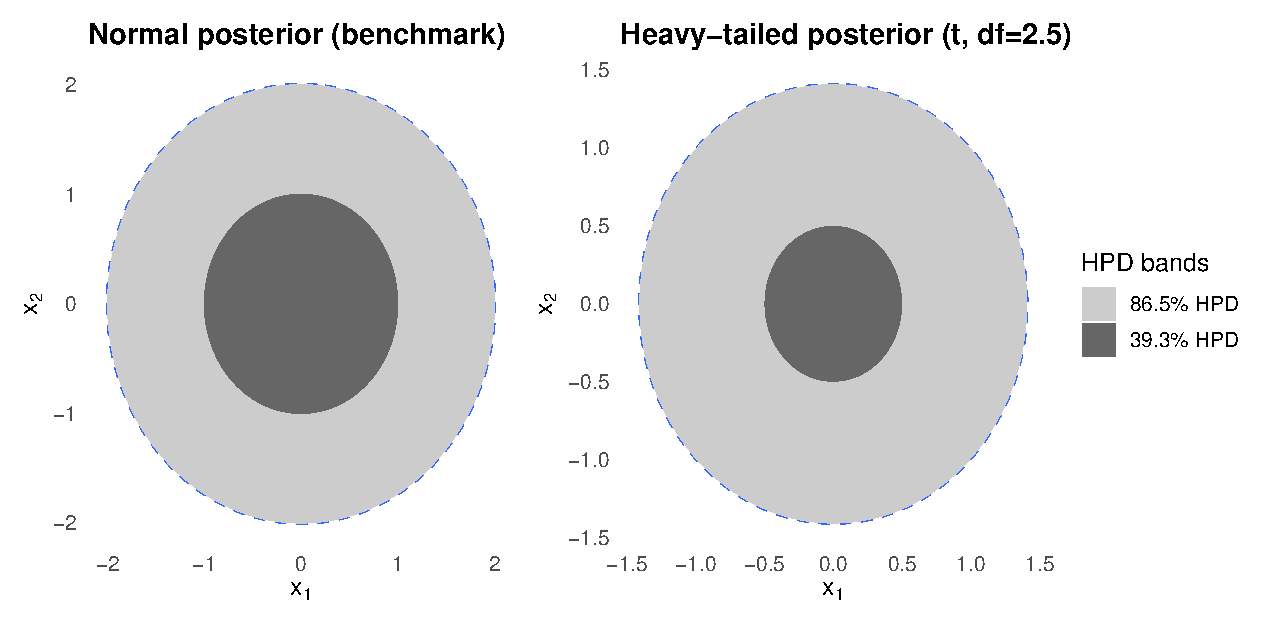
\includegraphics[height=5.5cm, width=0.8\textwidth]{images/hpd_normal_vs_student-t.pdf}
    \caption{{\small Illustrative HPD regions (39.3\% and 86.5\%) under a bivariate normal posterior (left) and a heavy-tailed $t$ distribution ($\text{df}=2.5$, right), both with $\mu=(0,0)$ and $\Sigma=I_2$.}}
    \label{fig:hpd-example}
\end{figure}
After obtaining the discretised posterior distribution, a natural next step is to extract the maximum a posteriori (MAP) estimate~\cite{gelman1995bayesian}. Within the grid framework, the MAP corresponds to the grid point $(\lambda^*, A^*)$ with the highest weight
\begin{equation}
    (\lambda^*, A^*) = \arg\max_{\lambda,A} \; p(\lambda,A \mid \mathcal D).
\end{equation}
This provides the most plausible parameter pair, which can serve as a reference point for pseudo-data generation and subsequent model checking~\cite{robert2007bayesian, gelman1995bayesian}.



\subsubsection{Marginalization of \texorpdfstring{$A$}{A} and Consistency Check}
\label{边际化章节}
The joint posterior $p(\lambda, A \mid \mathcal D)$ captures the dependence between the two parameters. To verify theoretical consistency with the original exponential model, we consider the marginal posterior of $\lambda$ obtained by integrating out $A$~\cite{gelman1995bayesian}.   

The central question is: does the marginal posterior of $\lambda$ coincide with that of the original exponential model (Equation~\ref{eq:16})? If so, this confirms that the extended model remains compatible with the original formulation and does not alter inference on $\lambda$.

Starting from Equation~\eqref{A_post}, we integrate out $A$~\cite{berger1999integrated}
\begin{equation}
    p(\lambda \mid \mathcal D)
= \int p(\lambda, A \mid \mathcal D)\,dA.
\end{equation}
Substituting, we obtain
\begin{equation}
    p(\lambda \mid \mathcal D)\;\propto\;\pi_\lambda(\lambda)\;\int L(\mathcal D \mid \lambda, A)\,\pi_A(A)\,dA.
    \label{eq:45}
\end{equation}
Thus, the integral in~\eqref{eq:45} reduces to a constant term independent of $\lambda$. 
Importantly, this constant absorbs both the $A$-dependent part of the likelihood and the prior $\pi_A(A)$, which means that the marginal posterior of $\lambda$ is independent of the prior choice for $A$. 
Therefore,
\begin{equation}
    L(\mathcal D \mid \lambda, A)
= \lambda^{\sum_i \delta_i}\;
e^{-\lambda \sum_i y_i}\;
\Bigg[
A^{-n}\,\prod_{i:\,\delta_i=1}(A-y_i)
\Bigg]\;\mathbf 1\{A \ge \max_i y_i\}.
\end{equation}
the integral in~\eqref{eq:45} separates into a constant term independent of $\lambda$. Thus,
\begin{align}
\label{eq:47}
p(\lambda \mid \mathcal{D})
&\propto \lambda^{\sum_i \delta_i}\,
e^{-\lambda \sum_i y_i}\,
\pi_\lambda(\lambda)\,
\underbrace{\int_{A \ge \max_i y_i}
A^{-n}\,\prod_{i:\,\delta_i=1}(A-y_i)\,\pi_A(A)\,dA}_{\text{constant, independent of }\lambda} \\[2pt]
&\propto \lambda^{\sum_i \delta_i}\, e^{-\lambda \sum_i y_i}\, \pi_{\lambda}(\lambda).
\end{align}
This is exactly the posterior distribution of the original exponential model (Equation~\ref{eq:16}).  

Numerically, the same result can be recovered by marginalizing over $A$ in the grid-based posterior representation: summing the normalized weights $\tilde w_{ij}$ along the $A$ dimension for each fixed $\lambda$ yields the marginal posterior of $\lambda$~\cite{ORMEROD201145, cowles2009reparameterized}. This numerical implementation matches the analytical derivation above, providing a computational-theoretical cross-check.

In summary, marginalizing $A$ restores the same posterior distribution for $\lambda$ as in the original exponential model. This demonstrates that the extended model is fully consistent with the original formulation: introducing $A$ enriches the model by explicitly representing the censoring window, while preserving the fundamental inference on $\lambda$.